%%
%%
%%
\subsection{\label{sec:videoStreams}Processing Video Streams}
\baustelle The processing of video streams is a recent application
that has been added to the \streams framework. The {\em streams-video}
package provides an implementation for streams of video frames in the
MJPEG format.

Several procssors have been added, e.g. for the extraction of features
from online video data. Features from videos might e.g. be indicating
commercial breaks or switches in scenes. 
cannot be derived from static EPG data or any other annotating data
sources. An overview about the video processing and the associated
scene and shot detection is outlined in Section
\ref{sec:videoFeatures}.

Researching the feature extraction from video data focuses on image
analysis of single video frames and the derived stream of features from
a series of such frames. The static feature extraction from images is
being investigated with the RapidMiner Image Mining Plugin \cite{Burget2010a}.

To support the online feature extraction from video data, the TUDO
group provides an image stream implemented for the \streams framework
which allows for applying processors to video frames in a streaming
manner. A sample of process definition for reading RAW video streams
is shown in Figure \ref{fig:videoXml}.

\begin{figure}[h!]
  \centering
  \begin{lstlisting}
    <container>

        <!--  This stream reads encoded JPG images from a file       -->    
        <stream  id="video" class="stream.io.MJpegImageStream"
                url="file:/Volumes/RamDisk/tagesschau.mjpeg.stream" />

        <process input="video">
             <!--  Add a 'frame:id' attribute, counting the frames    -->
             <CreateID key="frame:id" />
        
             <!--  Extract the average RGB channel values             -->
             <vista.video.ExtractAverageRGB />

             <!--  Plot the average red/green/blue channel values     -->         
             <WithKeys keys="frame:*" >
                  <stream.plotter.Plotter keys="frame:red:avg,frame:blue:avg,frame:green:avg"
                                       history="1000" />
             </WithKeys>
        </process>
    </container>
  \end{lstlisting}
  \caption{\label{fig:videoXml}A process definition for reading RAW
    video files encoded as a sequence of JPEG images. The processors
    used in this sample allow for extracting the average R/G/B channel
    values for each frame. The result is a 3-dimensional time series,
    emitting data at the usual frame rate of 25 samples per second.}
\end{figure}

\subsubsection*{Decoding Videos to MJPEG}
The format required for the {\ttfamily MJpegImageStream}
implementation to read video frames is a file of RAW decoded video
frames in JPEG image format. The stream implementation does not do the
decoding itself. Such a decoding can easily be derived from the open
source {\em MPlayer} tool, which is available for Linux, MacOS and
Windows. The {\em MPlayer} tool provides a standalone video decoder
called {\ttfamily mencoder} that can decode video streams and encode
these into various formats, including RAW JPEG sequence files.

For decoding a file {\ttfamily tagesschau.mp4}\footnote{The {\em
    Tagesschau} is a German news show, which provides hourly summaries
  of 90 seconds length. These can be downloaded from
  \url{http://www.tagesschau.de} and are used here for demonstration
  only.}, the {\ttfamily mencoder} needs to be invoked as:
\begin{verbatim}
   # mencoder tagesschau.mp4 -nosound -of rawvideo -o tagesschau.raw \
        -ovc lavc -lavcopts vcodec=mjpeg
\end{verbatim}
This will write a RAW JPEG sequence file to {\ttfamily tagesschau.raw}
which in turn can be read with the {\ttfamily MJpegImageStream} as shown
in Figure \ref{fig:videoXml}.

The {\ttfamily MJpegImageStream} will provide data items that contain
the raw byte array of the JPEG image in the {\ttfamily image:data}
attribute. This can further be used by processors to decode the original
bitmap image or display the image. The processor {\ttfamily AverageRGB}
decodes the image to a bitmap in order to compute the average color
channel values for the complete frame.

The {\ttfamily mencoder} tool as well as the \streams framework support
reading from standard input and writing to standard output. This allows
for decoding and processing live video streams from the Zattoo platform
later on.


\begin{figure}[h!]
  \centering
  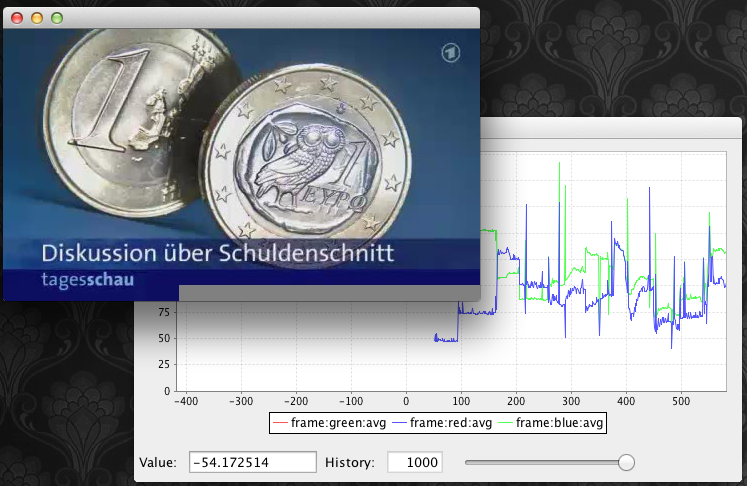
\includegraphics[scale=0.3]{graphics/video-stream.png}
  \caption{\label{fig:videoStreaming}The \streams framework
    continuously extracting average R/G/B channel values from a sample
    video while displaying the video frames to the screen.}
\end{figure}
